\documentclass[11pt]{article} 
\setlength{\oddsidemargin}{0.0in}
\setlength{\evensidemargin}{0.0in}
\setlength{\topmargin}{-0.25in}
\setlength{\headheight}{0in}
\setlength{\headsep}{0in}
\setlength{\textwidth}{6.5in}
\setlength{\textheight}{9.25in}
\setlength{\parindent}{0in}
\setlength{\parskip}{2mm}
\newcommand\tab[1][0.5cm]{\hspace*{#1}}
\usepackage{listings}
\usepackage{amsmath,amsfonts,amsthm, amssymb} % Math packages
\usepackage[utf8]{inputenc}
\usepackage{graphicx}
\usepackage{subcaption}
\usepackage{comment}

\title{ECS 189G Homework 2}
\author{Bochao Xin, Dianfeng Jiang, Melissa Goh, Shikun Huang}
\date{Due: 24 February 2020 (Monday)}

\begin{document}

\maketitle
\newpage
\tableofcontents
\newpage

\section{lm Model}
\subsection{Movienum}
Movienum will be our first predictor. But directly using movienum 
in lm function does not seem very promising, because movienum 
itself is only IDs for different movies and logically does not 
directly affect users' rating. Instead, we use movienum to 
calculate average rating of each individual movie. Then, we define 
movies with average ratings greater than or equal to 4.0 as 
"best movies" and define movies with average ratings less than or 
equal to 3.5 as "worst movies". Below is the code we used to do 
this job:
\begin{verbatim}
  # transform movienum to factor
  mov_factor <- as.factor(u.big$movienum) 
  levels <- levels(mov_factor)
  mov <- matrix(0,nrow = length(levels),ncol = 3)
  for (i in 1:length(levels)) {
    # find all the rows concerning the same movie
    movX <- u.big[mov_factor == levels[i],]
    average_rate <- mean(movX$rating)
    
    mov[i,1] <- as.numeric(levels[i])
    if(average_rate >= 4.0)
      mov[i,2] <- 1
    if(average_rate <= 3.5)
      mov[i,3] <- 1
  }
  mov <- as.data.frame(mov)
  names(mov) <- c("movienum","best_movie","worst_movie")
  
  # merge it back to data frame u.big later
  u.big <- merge(u.big, mov, by = "movienum", all.x = TRUE)
\end{verbatim}

Why did we do this? It comes from the intuition that some movies 
are just better than others. Those movies of high quality should 
receive higher scores than those of low quality. If most users 
speak highly of a certain movie, it proves that this movie is of 
high quality and tends to receive higher scores from future users, 
and vice versa.

\subsection{Usernum}
Our second predictor will be usernum. The way that we used to 
approach usernum is very similar to what we did for movienum. We 
use usernum to calculate average rating given by each individual 
user. Then, we define users who give average ratings less than or 
equal to 3.0 as "tough person" and define those who give average 
ratings greater than or equal to 4.0 as "nice person". Below is the 
code we used:
\begin{verbatim}
  usr_factor <- as.factor(u.big$usernum)
  levels <- levels(usr_factor)
  usr <- matrix(0,nrow=length(levels),ncol = 3)
  for (i in 1:length(levels)) {
    usrX <- u.big[usr_factor == levels[i],]
    average_rate <- mean(usrX$rating)
    usr[i,1] <- as.numeric(levels[i])
    
    if(average_rate >= 4.0)
      usr[i,2] <- 1
    if(average_rate <= 3.0)
      usr[i,3] <- 1
  }
  usr <- as.data.frame(usr)
  names(usr) <- c("usernum","nice_person","tough_person")
  u.big <- merge(u.big, usr, by = "usernum", all.x = TRUE)
\end{verbatim}

We did this based on the assumption that some users are just 
harsher than others, and they tend to give relative low ratings for 
movies they have seen. Also, some users are just more lenient than 
the ordinary, and they tend to give relative high ratings for 
movies.

\subsection{Genres}
Different kinds of movies should affect their ratings. Our first 
attempt is to use all genres as predictors. Below is the result:
\begin{verbatim}
Call:
lm(formula = as.formula(indexToStr(u.big, predictors)), data = u.big.trn)
Residuals:
    Min      1Q  Median      3Q     Max 
-3.1872 -0.6248  0.2613  0.6814  2.1056 
Coefficients:
             Estimate Std. Error t value Pr(>|t|)    
(Intercept)  3.383414   0.011023 306.929  < 2e-16 ***
unknown     -0.272303   0.369749  -0.736 0.461457    
Action      -0.085943   0.010808  -7.952 1.86e-15 ***
Adventure    0.080097   0.012636   6.339 2.33e-10 ***
Animation    0.353127   0.024639  14.332  < 2e-16 ***
Children    -0.219328   0.018535 -11.833  < 2e-16 ***
Comedy      -0.064776   0.010340  -6.265 3.75e-10 ***
Crime        0.087370   0.013776   6.342 2.27e-10 ***
Documentary  0.250434   0.042608   5.878 4.18e-09 ***
Drama        0.241360   0.010050  24.017  < 2e-16 ***
Fantasy     -0.204901   0.033054  -6.199 5.71e-10 ***
FilmNoir     0.392378   0.029256  13.412  < 2e-16 ***
Horror      -0.132379   0.016954  -7.808 5.85e-15 ***
Musical      0.066690   0.018914   3.526 0.000422 ***
Mystery      0.114597   0.017160   6.678 2.43e-11 ***
Romance      0.113899   0.009462  12.037  < 2e-16 ***
SciFi        0.095209   0.012179   7.818 5.44e-15 ***
Thriller     0.019249   0.010444   1.843 0.065324 .  
War          0.258046   0.013124  19.663  < 2e-16 ***
Western      0.190491   0.027305   6.976 3.05e-12 ***
---
Signif. codes:  0 ‘***’ 0.001 ‘**’ 0.01 ‘*’ 0.05 ‘.’ 0.1 ‘ ’ 1
Residual standard error: 1.109 on 94980 degrees of freedom
Multiple R-squared:  0.03026,	Adjusted R-squared:  0.03007 
F-statistic:   156 on 19 and 94980 DF,  p-value: < 2.2e-16
[1] 0.8778 # MAPE
\end{verbatim}

We can see from the above that not all genres has a great impact on
users' ratings. For example: the coefficient of "Action" movie is 
only $-0.0859$, meaning that whether a movie is action or not will
not affect people's ratings very much. Therefore, we could safely 
remove some genres from our predictors while preserving the 
accuracy of our predictions. Below are all the genres we 
included in our final lm model.
\begin{verbatim}
Call:
lm(formula = as.formula(indexToStr(u.big, predictors)), data = u.big.trn)
Residuals:
    Min      1Q  Median      3Q     Max 
-3.1460 -0.6262  0.2683  0.6501  2.0426 
Coefficients:
             Estimate Std. Error t value Pr(>|t|)    
(Intercept)  3.349864   0.006310 530.882  < 2e-16 ***
unknown     -0.238753   0.369962  -0.645    0.519    
Animation    0.377991   0.023603  16.015  < 2e-16 ***
Children    -0.188422   0.017653 -10.673  < 2e-16 ***
Documentary  0.282196   0.041782   6.754 1.45e-11 ***
Drama        0.276385   0.007848  35.218  < 2e-16 ***
Fantasy     -0.204048   0.032897  -6.203 5.58e-10 ***
FilmNoir     0.457673   0.028405  16.112  < 2e-16 ***
Horror      -0.117394   0.016462  -7.131 1.00e-12 ***
Mystery      0.140822   0.016722   8.421  < 2e-16 ***
Romance      0.105400   0.009358  11.263  < 2e-16 ***
SciFi        0.098830   0.011449   8.632  < 2e-16 ***
War          0.245364   0.012829  19.126  < 2e-16 ***
Western      0.169018   0.027010   6.258 3.93e-10 ***
---
Signif. codes:  0 ‘***’ 0.001 ‘**’ 0.01 ‘*’ 0.05 ‘.’ 0.1 ‘ ’ 1
Residual standard error: 1.11 on 94986 degrees of freedom
Multiple R-squared:  0.0285,	Adjusted R-squared:  0.02837 
F-statistic: 214.4 on 13 and 94986 DF,  p-value: < 2.2e-16
[1] 0.8778 # MAPE
\end{verbatim}

We found that even if we remove 6 different genres from our 
predictors, MAPE does not change.

\subsection{Occupations}
Our intuition to predicting ratings is based on factors that fundamentally represent the user's
personality. Some features we considered are age, usernum, and occupation. To elaborate on this,
we think that including usernum as a feature would let us know their rating based on how harshly
or leniently a user rates their movies, based on their user ID. 

\begin{figure}[ht!]
\begin{center}
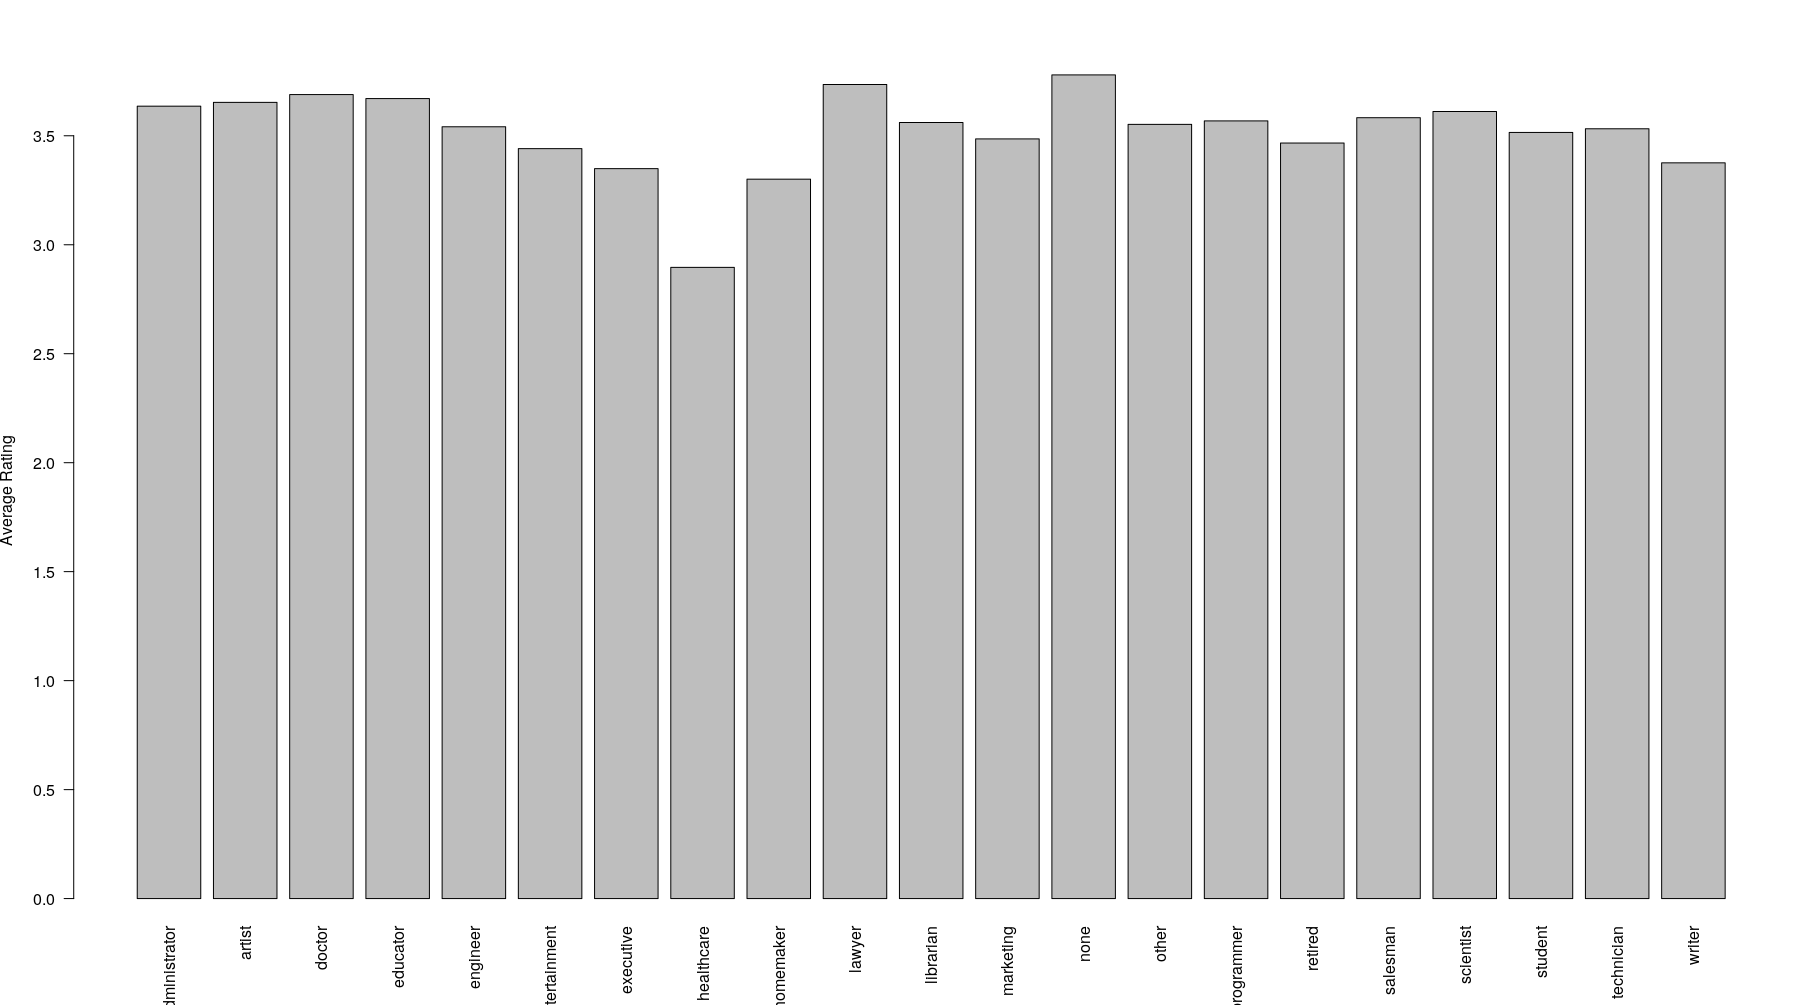
\includegraphics[width=0.8\textwidth]{ratingxocc.png}
\caption{Average Rating vs. Occupation}
\end{center}
\end{figure}

Intuitively, occupation reflects a person's personality. We plotted 
the average rating given by each occupation. As shown in the plot, 
the ratings are not very uniform, which would probably make 
Occupation a good feature to predict ratings. 
Our first attempt is simply using all occupations as our 
predictors. Here is the result.
\begin{verbatim}
Call:
lm(formula = as.formula(indexToStr(u.big, predictors)), data = u.big.trn)
Residuals:
    Min      1Q  Median      3Q     Max 
-2.7801 -0.5709  0.3527  0.5637  2.1075 
Coefficients:
                  Estimate Std. Error t value Pr(>|t|)    
(Intercept)        3.37842    0.01541 219.192  < 2e-16 ***
occ.administrator  0.25732    0.02034  12.649  < 2e-16 ***
occ.artist         0.26887    0.02836   9.480  < 2e-16 ***
occ.doctor         0.29994    0.05169   5.803 6.54e-09 ***
occ.educator       0.28936    0.01941  14.911  < 2e-16 ***
occ.engineer       0.16349    0.01995   8.194 2.56e-16 ***
occ.entertainment  0.05785    0.02944   1.965  0.04941 *  
occ.executive     -0.04073    0.02503  -1.627  0.10370    
occ.healthcare    -0.48588    0.02655 -18.299  < 2e-16 ***
occ.homemaker     -0.09729    0.06842  -1.422  0.15505    
occ.lawyer         0.36098    0.03489  10.345  < 2e-16 ***
occ.librarian      0.18277    0.02206   8.283  < 2e-16 ***
occ.marketing      0.10166    0.03016   3.371  0.00075 ***
occ.none           0.40169    0.04121   9.748  < 2e-16 ***
occ.other          0.16639    0.01899   8.763  < 2e-16 ***
occ.programmer     0.19248    0.02016   9.548  < 2e-16 ***
occ.retired        0.09592    0.03254   2.947  0.00321 ** 
occ.salesman       0.20450    0.04222   4.843 1.28e-06 ***
occ.scientist      0.23405    0.02960   7.908 2.64e-15 ***
occ.student        0.13405    0.01724   7.774 7.70e-15 ***
occ.technician     0.15457    0.02474   6.248 4.18e-10 ***
---
Signif. codes:  0 ‘***’ 0.001 ‘**’ 0.01 ‘*’ 0.05 ‘.’ 0.1 ‘ ’ 1
Residual standard error: 1.117 on 94979 degrees of freedom
Multiple R-squared:  0.01505,	Adjusted R-squared:  0.01484 
F-statistic: 72.55 on 20 and 94979 DF,  p-value: < 2.2e-16
[1] 0.8798 # MAPE
\end{verbatim}

Comparing this with Figure 1, we believe that ratings given by 
people of different occupations are around the same. But there are
two special cases. First, healthcare workers tend to give relative
low ratings compared to other occupations. Second, people whose 
occupation is none tend to give relative high ratings. Therefore,
the only two occupations we used as predictors are "healthcare" and
"none." Below is the result.
\begin{verbatim}
Call:
lm(formula = as.formula(indexToStr(u.big, predictors)), data = u.big.trn)
Residuals:
    Min      1Q  Median      3Q     Max 
-2.7801 -0.5441  0.4559  0.4559  2.1075 
Coefficients:
                Estimate Std. Error t value Pr(>|t|)    
(Intercept)     3.544111   0.003704 956.716  < 2e-16 ***
occ.healthcare -0.651561   0.021993 -29.626  < 2e-16 ***
occ.none        0.236006   0.038496   6.131 8.78e-10 ***
---
Signif. codes:  0 ‘***’ 0.001 ‘**’ 0.01 ‘*’ 0.05 ‘.’ 0.1 ‘ ’ 1
Residual standard error: 1.12 on 94997 degrees of freedom
Multiple R-squared:  0.009606,	Adjusted R-squared:  0.009585 
F-statistic: 460.7 on 2 and 94997 DF,  p-value: < 2.2e-16
[1] 0.8694 # MAPE
\end{verbatim}
We could see that using these two occupations as our predictors 
actually improves our result.
 
Since age likely affects
the kind of occupation a person has, we decided to use the interaction term `age` and `occ` to predicting
ratings. The MAPE obtained from this set of features is 0.8752.

\begin{verbatim}
    > lmout <- lm(rating ~ age*occ, data=trnSet)
    summary(lmout)
    > summary(lmout)
    
    Call:
    lm(formula = rating ~ age * occ, data = trnSet)
    
    Residuals:
        Min      1Q  Median      3Q     Max 
    -3.5559 -0.5763  0.3376  0.5374  2.8331 
    
    Coefficients:
                           Estimate Std. Error t value Pr(>|t|)    
    (Intercept)           3.3457294  0.0523707  63.885  < 2e-16 ***
    age                   0.0073463  0.0012955   5.670 1.43e-08 ***
    occartist            -0.6775732  0.1078113  -6.285 3.30e-10 ***
    occdoctor            -0.1125594  0.1831937  -0.614 0.538934    
    occeducator           0.3647334  0.0734661   4.965 6.89e-07 ***
    occengineer          -0.0359133  0.0688078  -0.522 0.601716    
    occentertainment      0.6526975  0.1318031   4.952 7.36e-07 ***
    occexecutive         -1.3817756  0.0913665 -15.123  < 2e-16 ***
    occhealthcare        -2.1325458  0.0901122 -23.665  < 2e-16 ***
    occhomemaker         -0.3012994  0.2346490  -1.284 0.199130    
    occlawyer             0.0806203  0.1262801   0.638 0.523199    
    occlibrarian          0.0534024  0.0785553   0.680 0.496629    
    occmarketing          0.3054019  0.1264570   2.415 0.015734 *  
    occnone               0.5380508  0.1263167   4.260 2.05e-05 ***
    occother              0.1970186  0.0646248   3.049 0.002299 ** 
    occprogrammer        -0.0590576  0.0695120  -0.850 0.395548    
    occretired           -0.3376369  0.4328787  -0.780 0.435404    
    occsalesman           0.1159735  0.1359053   0.853 0.393473    
    occscientist         -0.0424774  0.1416788  -0.300 0.764319    
    occstudent            0.2005008  0.0630880   3.178 0.001483 ** 
    occtechnician         0.2030625  0.0863610   2.351 0.018709 *  
    occwriter            -0.8011493  0.0768054 -10.431  < 2e-16 ***
    age:occartist         0.0247203  0.0032503   7.606 2.86e-14 ***
    age:occdoctor         0.0056768  0.0049181   1.154 0.248394    
    age:occeducator      -0.0083699  0.0017469  -4.791 1.66e-06 ***
    age:occengineer      -0.0007054  0.0017976  -0.392 0.694775    
    age:occentertainment -0.0267839  0.0043092  -6.216 5.14e-10 ***
    age:occexecutive      0.0302180  0.0023624  12.791  < 2e-16 ***
    age:occhealthcare     0.0360066  0.0022189  16.227  < 2e-16 ***
    age:occhomemaker      0.0009872  0.0068782   0.144 0.885874    
    age:occlawyer         0.0013949  0.0034506   0.404 0.686035    
    age:occlibrarian     -0.0031238  0.0019904  -1.569 0.116554    
    age:occmarketing     -0.0116446  0.0033326  -3.494 0.000476 ***
    age:occnone          -0.0114218  0.0045476  -2.512 0.012021 *  
    age:occother         -0.0071173  0.0017077  -4.168 3.08e-05 ***
    age:occprogrammer     0.0014500  0.0018701   0.775 0.438121    
    age:occretired        0.0001103  0.0070637   0.016 0.987546    
    age:occsalesman      -0.0038728  0.0037978  -1.020 0.307855    
    age:occscientist      0.0012039  0.0038758   0.311 0.756089    
    age:occstudent       -0.0085517  0.0020196  -4.234 2.29e-05 ***
    age:occtechnician    -0.0079412  0.0024493  -3.242 0.001186 ** 
    age:occwriter         0.0168032  0.0020383   8.244  < 2e-16 ***
    ---
    Signif. codes:  0 ‘***’ 0.001 ‘**’ 0.01 ‘*’ 0.05 ‘.’ 0.1 ‘ ’ 1
    
    Residual standard error: 1.109 on 94958 degrees of freedom
    Multiple R-squared:  0.02956,   Adjusted R-squared:  0.02914 
    F-statistic: 70.54 on 41 and 94958 DF,  p-value: < 2.2e-16
\end{verbatim}

\subsection{Interaction Terms}
We also explore some interaction terms. We think people of 
different occupations might have different preference for movies.
For example, artists might prefer drama and musical, and technician
might prefer science fiction. Therefoer, using interaction terms 
of occupations and genres might help us improve the accuracy of 
our prediction.

The first interaction term we include is $\textbf{executive} * \textbf{comedy}$.
\begin{figure}[ht!]
\begin{center}
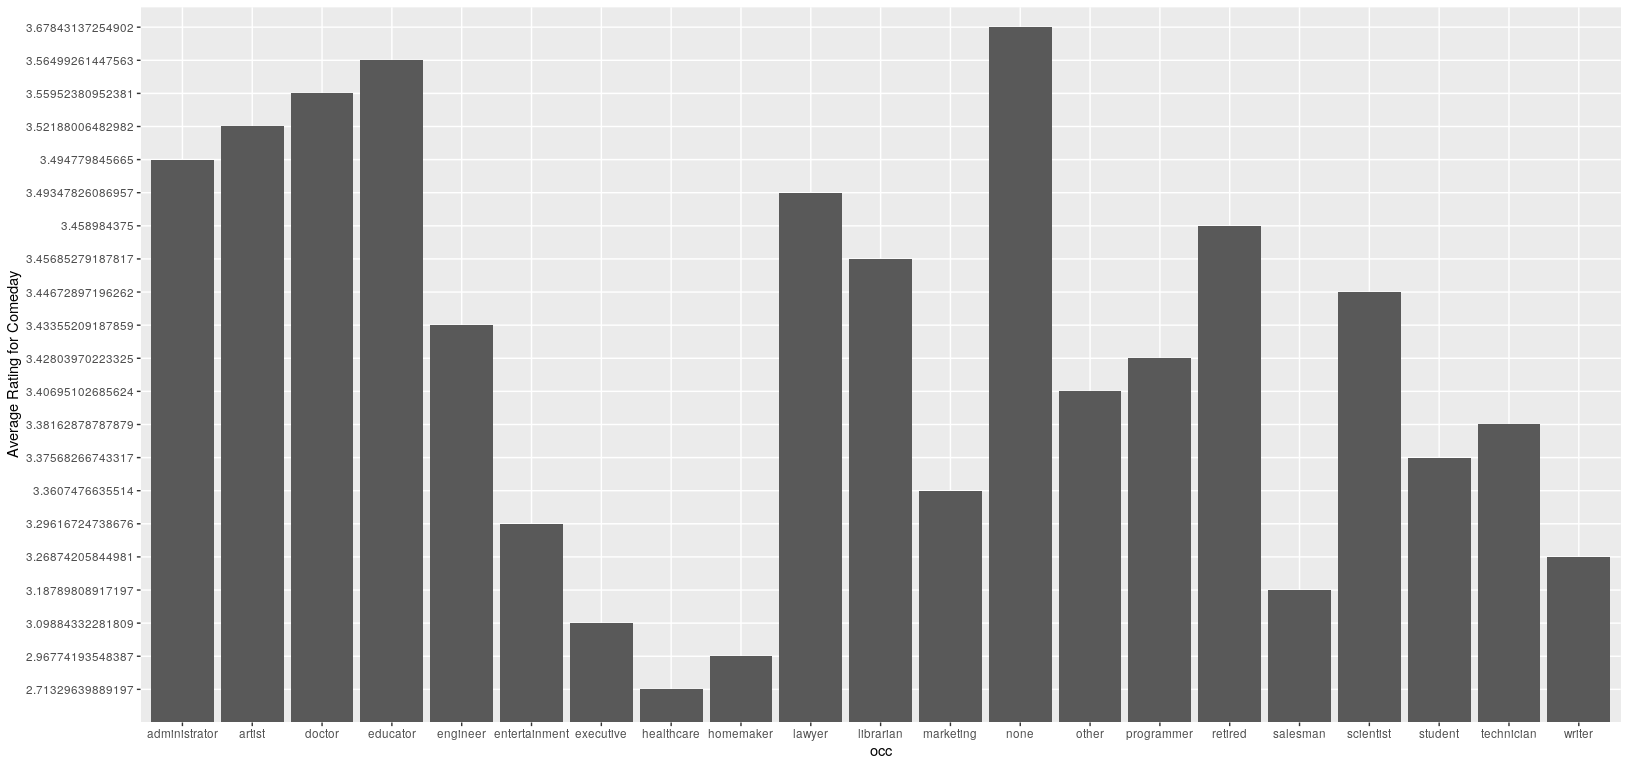
\includegraphics[width=\textwidth]{comedy_occ.png}
\caption{Average Rating for Comedy vs. Occupations}
\end{center}
\end{figure}

From the above plot, we find that executives tend to give low 
ratings for comedy. Therefore, we want to use $\textbf{executive} * \textbf{comedy}$ as 
one of interaction terms in our lm model.
\clearpage
The second interaction term we include is $\textbf{student} * \textbf{mystery}$.
\begin{figure}[ht!]
\begin{center}
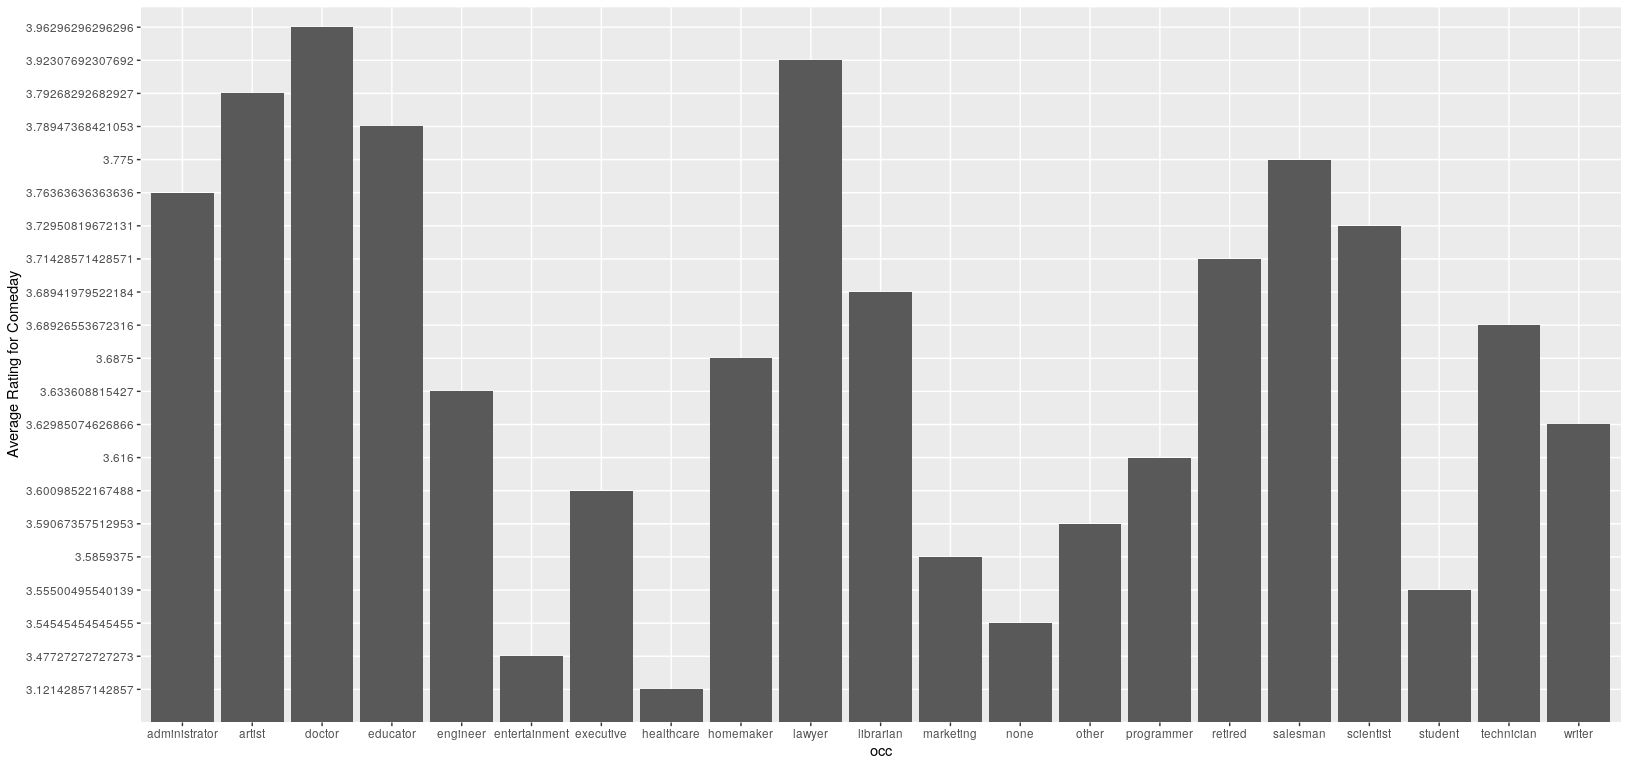
\includegraphics[width=\textwidth]{mystrey_student.png}
\caption{Average Rating for Mystery vs. Occupations}
\end{center}
\end{figure}

From the above plot, we find that students tend to give low 
ratings for mystery. Therefore, we want to use $\textbf{student} * \textbf{mystery}$ as one of interaction terms in our lm model.
\clearpage

Other interaction terms we include are $\textbf{artist} * \textbf{Sci-Fi}$ and $\textbf{writer} * \textbf{Sci-Fi}$.
\begin{figure}[ht!]
\begin{center}
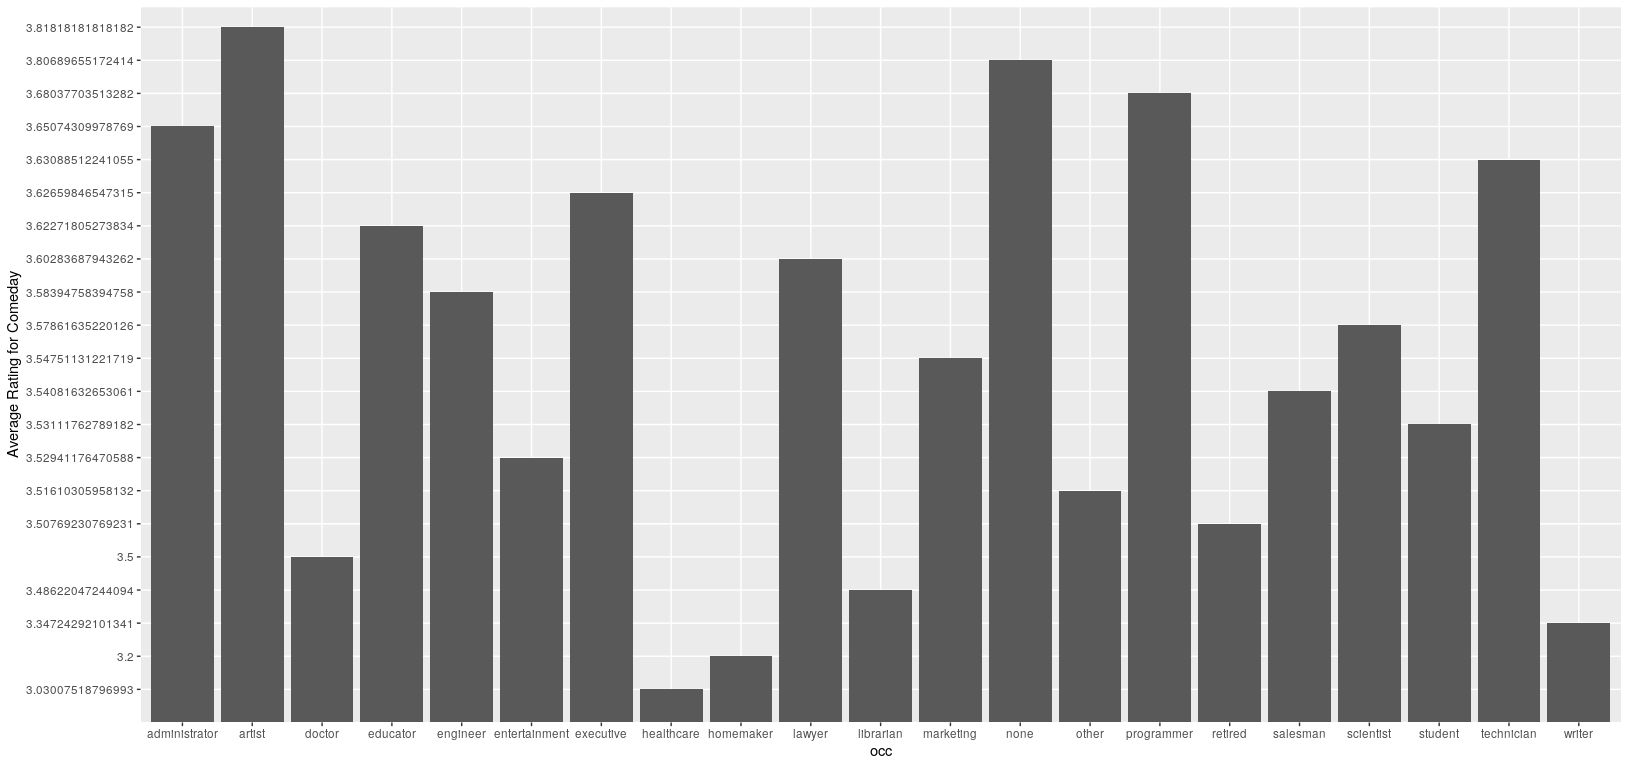
\includegraphics[width=\textwidth]{sci_fi.png}
\caption{Average Rating for Sci-Fi vs. Occupations}
\end{center}
\end{figure}
We figure out that artists give rather high ratings for science 
ficiton, while writers give rather low ratings for it. We expect
there will be a positive coefficient for $\textbf{artist} * \textbf{Sci-Fi}$ and a negative coefficient for $\textbf{writer} * \textbf{Sci-Fi}$.

The last interaction term we included is $\textbf{writer} * \textbf{Action}$.
\begin{figure}[ht!]
\begin{center}
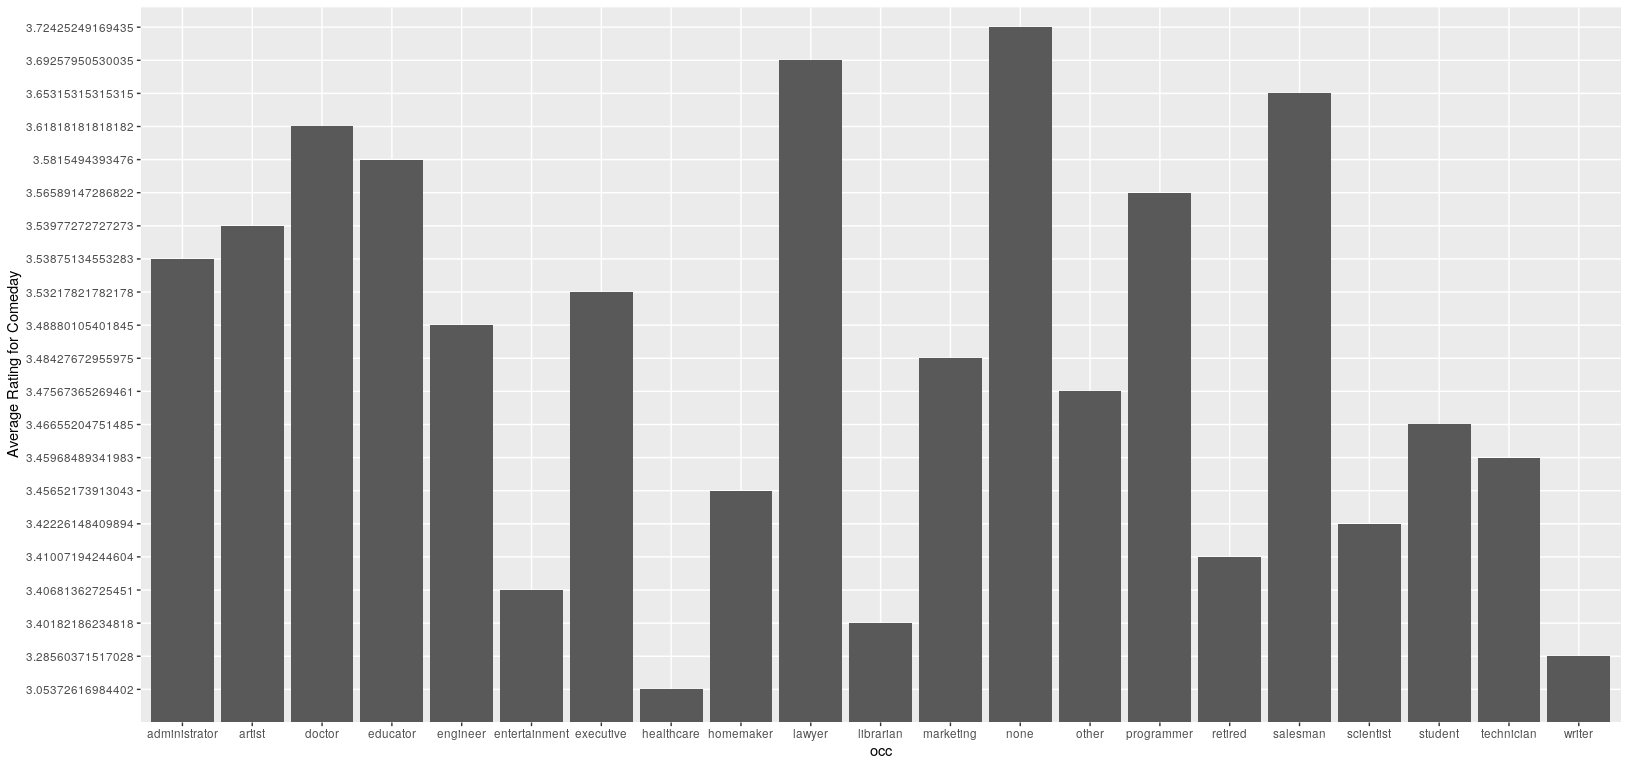
\includegraphics[width=\textwidth]{action.png}
\caption{Average Rating for Action Movies vs. Occupations}
\end{center}
\end{figure}
Writers tend to give quite low ratings for action movies. 
Therefore, using $\textbf{writer} * \textbf{Action}$ as interaction
term is highly likely to improve the accuracy of lm model.


\subsection{Final lm Model}
Our final model for lm will use usernum, movienum, some genres of 
movies, occupation of healthcare, occupation of none, and the above 
interaction terms as predictors. Below is the result of lm model. 
MAPE of this final model is 0.7446.

\begin{verbatim}
Call:
lm(formula = as.formula(indexToStr(u.big, predictors)), data = u.big.trn)
Residuals:
    Min      1Q  Median      3Q     Max 
-3.8027 -0.7197 -0.0117  0.8376  3.0302 
Coefficients:
                   Estimate Std. Error t value Pr(>|t|)    
(Intercept)       3.7036324  0.0076163 486.274  < 2e-16 ***
unknown           0.5043573  0.3282400   1.537  0.12441    
Animation         0.1714472  0.0209889   8.168 3.16e-16 ***
Children         -0.1277080  0.0156900  -8.139 4.02e-16 ***
Documentary       0.0707132  0.0371344   1.904  0.05688 .  
Drama             0.0621791  0.0072294   8.601  < 2e-16 ***
Fantasy           0.0007598  0.0290901   0.026  0.97916    
FilmNoir          0.0254993  0.0258373   0.987  0.32368    
Horror           -0.0290689  0.0146480  -1.985  0.04720 *  
Mystery           0.0556986  0.0165068   3.374  0.00074 ***
Romance           0.0373975  0.0083367   4.486 7.27e-06 ***
SciFi             0.0294848  0.0105000   2.808  0.00498 ** 
War               0.0294362  0.0116348   2.530  0.01141 *  
Western           0.0940044  0.0239513   3.925 8.69e-05 ***
occ.healthcare   -0.2450486  0.0200063 -12.249  < 2e-16 ***
occ.none          0.4087876  0.0338730  12.068  < 2e-16 ***
executive_comedy -0.2558763  0.0333103  -7.682 1.59e-14 ***
student_mystrery  0.0224079  0.0355071   0.631  0.52799    
artist_SciFi      0.0346920  0.0579341   0.599  0.54930    
writer_SciFi     -0.0525257  0.0442267  -1.188  0.23498    
writer_action    -0.0963854  0.0314375  -3.066  0.00217 ** 
best_movie        0.3737968  0.0094795  39.432  < 2e-16 ***
worst_movie      -0.6264494  0.0073858 -84.818  < 2e-16 ***
nice_person       0.5612674  0.0098445  57.013  < 2e-16 ***
tough_person     -0.7346390  0.0110443 -66.517  < 2e-16 ***
---
Signif. codes:  0 ‘***’ 0.001 ‘**’ 0.01 ‘*’ 0.05 ‘.’ 0.1 ‘ ’ 1
Residual standard error: 0.9845 on 94975 degrees of freedom
Multiple R-squared:  0.2359,	Adjusted R-squared:  0.2357 
F-statistic:  1222 on 24 and 94975 DF,  p-value: < 2.2e-16
[1] 0.7446
\end{verbatim}

\section{Nmf Model}
\tab{}In the nmf model, we input usernum, movienum, and rating as the input of the training set of the recosystem()'s \$train() function.
\\*
\subsection{Default}
\tab{}We ran the \$train() function once with default tuning parameters beside the nmf = TRUE because we want the function to use nmf method instead of svd, and we want to see the MAPE() result with default settings so we could have a standard later on when we tune it.
\begin{verbatim}
     ty$train(trnst, opts = list(nmf = TRUE))
iter      tr_rmse          obj
   0       1.2098   2.0622e+05
   1       0.9580   1.5430e+05
   2       0.9451   1.5210e+05
   3       0.9385   1.5091e+05
   4       0.9329   1.5026e+05
   5       0.9265   1.4943e+05
   6       0.9202   1.4877e+05
   7       0.9138   1.4803e+05
   8       0.9085   1.4750e+05
   9       0.9043   1.4687e+05
  10       0.9005   1.4655e+05
  11       0.8971   1.4604e+05
  12       0.8948   1.4595e+05
  13       0.8921   1.4552e+05
  14       0.8901   1.4522e+05
  15       0.8886   1.4526e+05
  16       0.8866   1.4489e+05
  17       0.8852   1.4491e+05
  18       0.8839   1.4488e+05
  19       0.8820   1.4446e+05
> res <- ty$predict(tststX, out_memory())
> MAPE(res, tststY)
[1] 0.7329318
\end{verbatim}

\tab{}The MAPE() result for the nmf model is 0.7329318, which is not really "bad" consider it is already lower than our best lm model.

\subsection{Tune}
\tab{} To increase the accuracy of our model, we used \$tune() and \$train() function together to tune the tuning parameters in the opts. Often, we utilized \$tune() function in the beginning to traverse a large scale of values since it automatically pick the best values from the input vector. After that, we used \$train() to test a small amounts of values that varies a little from the best values the \$tune() function gave us. We choose this method because running \$tune() function generally took longer time to receive the result than retrain the model with a new parameter, and the running time of \$tune() will increase drastically when we increased the amount of values we wanted to guess. Thus, it's more time efficient for us to apply.
\subsubsection{Dim}
\tab{}We first tried different \textbf{\underline{dim}}, and see how the MAPE() result changed. We noticed that there would be an "optimal" number within a region, like a "local" optimize point so the result would be the lowest. After tested different dim under multiple distinct interval and considered the rule of thumb that $p << \sqrt{n}$, we choose dim=25:
\\*
\begin{verbatim}
    ty$train(trnst, opts = list(dim = 25, nmf = TRUE))
iter      tr_rmse          obj
   0       1.2686   2.2040e+05
   1       0.9644   1.5517e+05
   2       0.9471   1.5257e+05
   3       0.9349   1.5094e+05
   4       0.9247   1.4965e+05
   5       0.9160   1.4854e+05
   6       0.9091   1.4795e+05
   7       0.9027   1.4713e+05
   8       0.8969   1.4667e+05
   9       0.8915   1.4606e+05
  10       0.8863   1.4541e+05
  11       0.8822   1.4527e+05
  12       0.8777   1.4483e+05
  13       0.8739   1.4457e+05
  14       0.8701   1.4422e+05
  15       0.8664   1.4381e+05
  16       0.8631   1.4360e+05
  17       0.8601   1.4342e+05
  18       0.8570   1.4321e+05
  19       0.8539   1.4264e+05
> res <- ty$predict(tststX, out_memory())
> MAPE(res, tststY)
[1] 0.7234832
\end{verbatim}
This improve the MAPE() result for 0.01 compared to the default one.

\subsubsection{Niter}
\tab{}Then, we tried different \textbf{\underline{niter}} since we discover the accuracy will increase as this parameter increase. But there is a asymptomatic ceiling for this parameter, which the improvement would not be noticeable or even could decrease the accuracy if we keep increasing it. Thus, after we played around with it, we set niter=80 as it improve our result for another 0.01.
\begin{verbatim}
    ty$train(trnst, opts = list(dim = 25, niter= 80, nmf = TRUE))
iter      tr_rmse          obj
   0       1.2686   2.2040e+05
   1       0.9644   1.5517e+05
   2       0.9471   1.5257e+05
   3       0.9349   1.5094e+05
   4       0.9247   1.4965e+05
   5       0.9160   1.4854e+05
   6       0.9091   1.4795e+05
   7       0.9027   1.4713e+05
   8       0.8969   1.4667e+05
   9       0.8915   1.4606e+05
  10       0.8863   1.4541e+05
  11       0.8822   1.4527e+05
  12       0.8777   1.4483e+05
  13       0.8739   1.4457e+05
  14       0.8701   1.4422e+05
  15       0.8664   1.4381e+05
  16       0.8631   1.4360e+05
  17       0.8601   1.4342e+05
  18       0.8570   1.4321e+05
  19       0.8539   1.4264e+05
  20       0.8516   1.4273e+05
...
  70       0.7862   1.3854e+05
  71       0.7854   1.3845e+05
  72       0.7850   1.3851e+05
  73       0.7841   1.3836e+05
  74       0.7835   1.3830e+05
  75       0.7829   1.3829e+05
  76       0.7824   1.3827e+05
  77       0.7817   1.3822e+05
  78       0.7814   1.3830e+05
  79       0.7805   1.3817e+05
> res <- ty$predict(tststX, out_memory())
> MAPE(res, tststY)
[1] 0.7139921
\end{verbatim}
\tab{}Until this point, our nmf model's MAPE() result is 0.7139921 which improve by 0.018 compares to the original model with default tuning parameter. 

\subsubsection{Lrate}
\tab{}p.s. After Monday's lecture that discussed about the letter, we've done some search on the learning rate which is the step size between each iteration. We believe that the lrate parameter has the potential to further improve our model's accuracy.
\begin{verbatim}
    ty$train(trnst, opts = list(dim = 25, niter= 80, lrate = 0.13, nmf = TRUE))
iter      tr_rmse          obj
   0       1.1953   2.0343e+05
   1       0.9669   1.5572e+05
   2       0.9492   1.5317e+05
   3       0.9358   1.5138e+05
   4       0.9257   1.5008e+05
   5       0.9172   1.4902e+05
   6       0.9102   1.4850e+05
   7       0.9034   1.4764e+05
   8       0.8971   1.4716e+05
   9       0.8910   1.4648e+05
  10       0.8852   1.4576e+05
  11       0.8806   1.4561e+05
  12       0.8757   1.4520e+05
  13       0.8714   1.4490e+05
  14       0.8672   1.4451e+05
  15       0.8631   1.4408e+05
  16       0.8593   1.4383e+05
  17       0.8560   1.4366e+05
  18       0.8525   1.4338e+05
  19       0.8491   1.4276e+05
  20       0.8463   1.4286e+05
...
  70       0.7745   1.3830e+05
  71       0.7737   1.3821e+05
  72       0.7733   1.3829e+05
  73       0.7722   1.3809e+05
  74       0.7715   1.3803e+05
  75       0.7709   1.3801e+05
  76       0.7705   1.3802e+05
  77       0.7697   1.3795e+05
  78       0.7693   1.3805e+05
  79       0.7684   1.3791e+05
> res <- ty$predict(tststX, out_memory())
> MAPE(res, tststY)
[1] 0.7130311
\end{verbatim}
\tab{}Indeed, it turns out that the MAPE() result become 0.7130311. which is 0.001 better than our previous model with lrate default to 0.1.

\subsection{Some other attempts}
\tab{}In addition, we also tried plugging in different predictors to user\_index and item\_index to see what happens to the predicting results. But the accuracy of the combinations we have tested are all worse than the original one with usernum and movienum. We think that since we are predicting existing users and movies, movienum and usernum should be the most dominant predictor in this model. Thus, we still stick to our previous best model.

\subsection{Final Nmf Model}
\tab{}Combining all these tuning parameters we've tried, our final model was yield with opts = list(dim = 25, niter= 80, lrate = 0.13, nmf = TRUE), and this gave us 0.7130311 in the MAPE() result, and it's 0.02 better in accuracy than the original default model.


\section{Contributions}
\subsection{Bochao Xin}
I worked primarily on lm model, and also tried a few nmf models. I 
developed helper function \textbf{Initalization()}, 
\textbf{roundToNearestInt}, and \textbf{IndexToStr()}. I proposed 
to add \textbf{movienum}, and \textbf{usernum} to predictors, and 
developed the way to use them in lm model. I explored which 
occupations and genres we should add to our lm model. I tested the 
relationship between occupations and genres and added those five 
interaction terms into our lm model. Actually, I also tested the 
relationship between age and genres because I think people of 
different ages might have different preference for movies. But I
found that there is no strong relationship between them.
I also wrote \textbf{lmFinalModel()} function, and most(not all!) of the report for lm model.

\subsection{Melissa Goh}
I tested a few models in lm and the best one that I found was 
age*occ (Appendix, 3.2.1). I wrote the function \textbf{avgOccRating},
and plotted the average movie rating that each group of occupation gives.
I contributed to the lm section of the report explaining why I did this.

\subsection{Shikun Huang}
I tried a few combination of lm models and wrote a very small part of 
description about the use of the dims parameter of tune function in the appendix.
To be honest, my teammates also contributed to help me to understand
the materials.

\subsection{Dianfeng Jiang}
I worked both on lm model and nmf model. In lm model, I tested serveral 
different models without interaction terms at first. After that, I was mainly 
exploring the interaction terms which corresponding to the \textbf{Ex-model1-10} 
in the appendix. And, I tried to filter those that have a coefficient that are >0.1 
\textbf{(Ex-model4, Ex-model10)} and built a new model based on them. I developed several
variances of Bochao's \textbf{IndexToStr()} function to help me deploy multiple interaction 
terms within one model and see their effectiveness. 
In nmf model, I applied the method I described in the beginning of the \textbf{Tune} section 
that used both \$train() and \$tune() together to find the best model. I wrote the \textbf{nmf\_gen()} 
function based on the best model I had found, and the \textbf{nmfFinalModel()}. I also wrote the 
report for the nmf model.


\section{Appendix}
\subsection{Helper Functions}
\subsubsection{Initialization}
This function is used to prepare the u.big dataset used throughout
this assignment.
\begin{verbatim}
# form the database we are gonna use for Hwk2
initialization <- function() {
	library(regtools)
	ratings <- read.table('ml-100k/u.data')
	names(ratings) <- c('usernum', 'movienum', 'rating', 'transID')
	demog <- read.table('ml-100k/u.user', sep='|')
	names(demog) <- c('usernum', 'age', 'gender', 'occ', 'ZIP')
	u.big <- merge(ratings,demog,by.x=1,by.y=1)
	movies <- read.csv("ml-100k/u.item", sep="|", check.names=FALSE, header=FALSE, fill=TRUE)
	genres <- read.csv("ml-100k/u.genre", sep="|", check.names=FALSE, header=FALSE)
	movies <- movies[,c(-2:-5)]
	names(movies) <- c('movienum', as.character(genres[,1]))
	u.big <- merge(u.big, movies, by = "movienum", all.x = TRUE)
	u.big <- u.big[order(u.big$usernum, u.big$movienum),]
	# print(sum(is.na(u.big$ZIP)))
	# how to deal with ZIP
	zips <- as.character(u.big$ZIP)
	zips <- substr(zips,1,2)
	u.big$ZIP <- as.factor(zips)
	# print(sum(is.na(u.big$ZIP)))
	return(u.big)
}
\end{verbatim}
\subsubsection{Round To the Nearest Int}
This function is used to convert result to the nearest int.
\begin{verbatim}
roundToNearestInt <- function(vec){
  a <- vec %% 1
  vec[a >= 0.5] = ceiling(vec[a >= 0.5])
  vec[a < 0.5] = floor(vec[a < 0.5])
  return(vec)
}
\end{verbatim}
\subsubsection{dims variable in tune}
why the dims parameter in tune function is a vector? it is because the tune function will perform cross validation,
and dims will hold different options of  latent factors, so tune function can find the dim that has the best validation error.

\subsubsection{Index To String}
This function is used to convert the input columns into the string
that will be used in lm model. We want this function so that we don't need to manually type all the predictors by ourselves.
\begin{verbatim}
indexToStr <- function(u.big, index){
  str <- paste("rating ", "~",
        paste(' ', colnames(u.big)[index], ' ', sep = "", collapse = "+"),
        sep = "")
  return(str)
}
> u.big <- initialization()
> indexToStr(u.big, c(1,2,9:27))
[1] "rating ~ movienum + usernum + unknown + Action + Adventure + 
Animation + Children's + Comedy + Crime + Documentary + Drama + 
Fantasy + Film-Noir + Horror + Musical + Mystery + Romance + Sci-Fi 
+ Thriller + War + Western "
\end{verbatim}

\subsection{Other Lm Models Attempted}
\subsubsection{Ex-model1}
\textbf{\underline{(Age$*$occ)}}
\begin{verbatim}
Call:
lm(formula = rating ~ age * occ, data = u.big.trn)
Coefficients:
         (Intercept)                   age             occartist             occdoctor  
           3.3457294             0.0073463            -0.6775732            -0.1125594  
         occeducator           occengineer      occentertainment          occexecutive  
           0.3647334            -0.0359133             0.6526975            -1.3817756  
       occhealthcare          occhomemaker             occlawyer          occlibrarian  
          -2.1325458            -0.3012994             0.0806203             0.0534024  
        occmarketing               occnone              occother         occprogrammer  
           0.3054019             0.5380508             0.1970186            -0.0590576  
          occretired           occsalesman          occscientist            occstudent  
          -0.3376369             0.1159735            -0.0424774             0.2005008  
       occtechnician             occwriter         age:occartist         age:occdoctor  
           0.2030625            -0.8011493             0.0247203             0.0056768  
     age:occeducator       age:occengineer  age:occentertainment      age:occexecutive  
          -0.0083699            -0.0007054            -0.0267839             0.0302180  
   age:occhealthcare      age:occhomemaker         age:occlawyer      age:occlibrarian  
           0.0360066             0.0009872             0.0013949            -0.0031238  
    age:occmarketing           age:occnone          age:occother     age:occprogrammer  
          -0.0116446            -0.0114218            -0.0071173             0.0014500  
      age:occretired       age:occsalesman      age:occscientist        age:occstudent  
           0.0001103            -0.0038728             0.0012039            -0.0085517  
   age:occtechnician         age:occwriter  
          -0.0079412             0.0168032  
\end{verbatim}

\subsubsection{Ex-model2}
\textbf{\underline{(Age$*$Gender)}}
\begin{verbatim}
Call:
lm(formula = rating ~ age * dum_gen.F, data = u.big.trn)
Coefficients:
  (Intercept)            age      dum_gen.F  age:dum_gen.F  
    3.3512072      0.0053591      0.0303178     -0.0007553 
\end{verbatim}

\subsubsection{Ex-model3}
\textbf{\underline{(movienum+usernum+genre+age$*$occ)}}
\begin{verbatim}
    Call:
lm(formula = as.formula(indexToStr3(u.big, c(1, 2, 9:28), 5, 
    c(29:48))), data = u.big.trn)
Coefficients:
              (Intercept)                   movienum                    usernum  
                2.871e+00                 -6.169e-04                 -1.763e-05  
                  unknown                     Action                  Adventure  
               -3.004e-01                 -1.365e-01                  6.568e-02  
                Animation                   Children                     Comedy  
                3.160e-01                 -2.639e-01                 -1.191e-01  
                    Crime                Documentary                      Drama  
               -1.454e-02                  3.287e-01                  1.934e-01  
                  Fantasy                   FilmNoir                     Horror  
               -7.335e-02                  4.129e-01                 -1.593e-01  
                  Musical                    Mystery                    Romance  
                1.462e-02                  8.864e-02                  9.009e-02  
                    SciFi                   Thriller                        War  
               -9.738e-03                 -8.634e-03                  1.878e-01  
                  Western                  dum_gen.F                        age  
                1.147e-01                  6.444e-02                  2.085e-02  
    dum_occ.administrator             dum_occ.artist             dum_occ.doctor  
                6.942e-01                  1.401e-01                  5.213e-01  
         dum_occ.educator           dum_occ.engineer      dum_occ.entertainment  
                9.816e-01                  6.605e-01                  1.369e+00  
        dum_occ.executive         dum_occ.healthcare          dum_occ.homemaker  
               -4.614e-01                 -1.263e+00                  5.101e-01  
           dum_occ.lawyer          dum_occ.librarian          dum_occ.marketing  
                9.730e-01                  7.088e-01                  9.007e-01  
             dum_occ.none              dum_occ.other         dum_occ.programmer  
                1.387e+00                  9.364e-01                  6.820e-01  
          dum_occ.retired           dum_occ.salesman          dum_occ.scientist  
                7.286e-01                  9.490e-01                  5.339e-01  
          dum_occ.student         dum_occ.technician  age:dum_occ.administrator  
                9.896e-01                  9.035e-01                 -1.456e-02  
       age:dum_occ.artist         age:dum_occ.doctor       age:dum_occ.educator  
                5.738e-03                 -6.614e-03                 -2.104e-02  
     age:dum_occ.engineer  age:dum_occ.entertainment      age:dum_occ.executive  
               -1.462e-02                 -4.069e-02                  1.112e-02  
   age:dum_occ.healthcare      age:dum_occ.homemaker         age:dum_occ.lawyer  
                1.849e-02                 -1.681e-02                 -1.823e-02  
    age:dum_occ.librarian      age:dum_occ.marketing           age:dum_occ.none  
               -1.721e-02                 -2.367e-02                 -2.955e-02  
        age:dum_occ.other     age:dum_occ.programmer        age:dum_occ.retired  
               -2.260e-02                 -1.325e-02                 -1.949e-02  
     age:dum_occ.salesman      age:dum_occ.scientist        age:dum_occ.student  
               -2.208e-02                 -1.081e-02                 -2.567e-02  
   age:dum_occ.technician  
               -2.213e-02  
> MAPE(res, u.big.tstY)
[1] 0.8759136
\end{verbatim}

\subsubsection{Ex-model4}
\textbf{\underline{(movienum+usernum+genre+age$*$occ(filtered))}}
\begin{verbatim}
> ty <- lmout$coefficients[which(lmout$coefficients>0.1)]
> ty
          (Intercept)             Animation           Documentary                 Drama 
            2.8709570             0.3160384             0.3287317             0.1934401 
             FilmNoir                   War               Western dum_occ.administrator 
            0.4129342             0.1877643             0.1146586             0.6941661 
       dum_occ.artist        dum_occ.doctor      dum_occ.educator      dum_occ.engineer 
            0.1401388             0.5212673             0.9816013             0.6605198 
dum_occ.entertainment     dum_occ.homemaker        dum_occ.lawyer     dum_occ.librarian 
            1.3692947             0.5100636             0.9730293             0.7088333 
    dum_occ.marketing          dum_occ.none         dum_occ.other    dum_occ.programmer 
            0.9006979             1.3874222             0.9364326             0.6820366 
      dum_occ.retired      dum_occ.salesman     dum_occ.scientist       dum_occ.student 
            0.7285785             0.9489834             0.5338967             0.9896029 
   dum_occ.technician 
            0.9035196
> MAPE(res, u.big.tstY)
[1] 0.9175987
\end{verbatim}


\subsubsection{Ex-model5}
\textbf{\underline{(movienum+usernum+gender$*$occ)}}
\begin{verbatim}
Call:
lm(formula = as.formula(indexToStr3(u.big, c(1, 2, 9:27), 28, 
    c(29:48))), data = u.big.trn)
Coefficients:
                    (Intercept)                         movienum  
                      3.404e+00                       -6.280e-04  
                        usernum                          unknown  
                     -5.953e-06                       -3.073e-01  
                         Action                        Adventure  
                     -1.390e-01                        6.260e-02  
                      Animation                         Children  
                      3.082e-01                       -2.727e-01  
                         Comedy                            Crime  
                     -1.173e-01                       -1.483e-02  
                    Documentary                            Drama  
                      3.411e-01                        1.980e-01  
                        Fantasy                         FilmNoir  
                     -7.536e-02                        4.177e-01  
                         Horror                          Musical  
                     -1.726e-01                        1.875e-02  
                        Mystery                          Romance  
                      9.533e-02                        9.008e-02  
                          SciFi                         Thriller  
                     -1.351e-02                       -8.723e-03  
                            War                          Western  
                      1.918e-01                        1.185e-01  
                      dum_gen.F            dum_occ.administrator  
                      5.136e-01                        3.615e-01  
                 dum_occ.artist                   dum_occ.doctor  
                      6.371e-01                        4.929e-01  
               dum_occ.educator                 dum_occ.engineer  
                      4.508e-01                        3.389e-01  
          dum_occ.entertainment                dum_occ.executive  
                      2.743e-01                        1.517e-01  
             dum_occ.healthcare                dum_occ.homemaker  
                      4.449e-01                        2.940e-01  
                 dum_occ.lawyer                dum_occ.librarian  
                      5.399e-01                        3.214e-01  
              dum_occ.marketing                     dum_occ.none  
                      2.674e-01                        7.805e-01  
                  dum_occ.other               dum_occ.programmer  
                      3.834e-01                        4.010e-01  
                dum_occ.retired                 dum_occ.salesman  
                      2.919e-01                        2.262e-01  
              dum_occ.scientist                  dum_occ.student  
                      3.845e-01                        3.322e-01  
             dum_occ.technician  dum_gen.F:dum_occ.administrator  
                      3.365e-01                       -3.213e-01  
       dum_gen.F:dum_occ.artist         dum_gen.F:dum_occ.doctor  
                     -9.638e-01                               NA  
     dum_gen.F:dum_occ.educator       dum_gen.F:dum_occ.engineer  
                     -4.925e-01                       -3.686e-01  
dum_gen.F:dum_occ.entertainment      dum_gen.F:dum_occ.executive  
                     -5.271e-01                       -9.148e-02  
   dum_gen.F:dum_occ.healthcare      dum_gen.F:dum_occ.homemaker  
                     -1.315e+00                       -6.567e-01  
       dum_gen.F:dum_occ.lawyer      dum_gen.F:dum_occ.librarian  
                     -6.624e-01                       -4.710e-01  
    dum_gen.F:dum_occ.marketing           dum_gen.F:dum_occ.none  
                     -4.660e-01                       -7.941e-01  
        dum_gen.F:dum_occ.other     dum_gen.F:dum_occ.programmer  
                     -5.624e-01                       -5.515e-01  
      dum_gen.F:dum_occ.retired       dum_gen.F:dum_occ.salesman  
                     -7.605e-01                       -7.597e-02  
    dum_gen.F:dum_occ.scientist        dum_gen.F:dum_occ.student  
                     -9.140e-01                       -3.829e-01  
   dum_gen.F:dum_occ.technician  
                     -7.121e-01  
> MAPE(res, u.big.tstY)
[1] 0.8788762
\end{verbatim}

\subsubsection{Ex-model6}
\textbf{\underline{(movienum+usernum+gender$*$genre)}}
\begin{verbatim}
    Call:
lm(formula = as.formula(indexToStr3(u.big, c(1, 2), 28, c(9:27))), 
    data = u.big.trn)
Coefficients:
          (Intercept)               movienum                usernum              dum_gen.F  
            3.771e+00             -6.598e-04             -3.415e-05              2.399e-02  
              unknown                 Action              Adventure              Animation  
           -3.673e-01             -1.420e-01              6.268e-02              3.331e-01  
             Children                 Comedy                  Crime            Documentary  
           -3.090e-01             -1.180e-01             -5.365e-03              3.198e-01  
                Drama                Fantasy               FilmNoir                 Horror  
            2.038e-01             -5.268e-02              4.587e-01             -1.612e-01  
              Musical                Mystery                Romance                  SciFi  
           -3.301e-03              1.199e-01              7.863e-02              9.563e-03  
             Thriller                    War                Western      dum_gen.F:unknown  
           -1.026e-02              2.068e-01              1.639e-01              2.535e-01  
     dum_gen.F:Action    dum_gen.F:Adventure    dum_gen.F:Animation     dum_gen.F:Children  
            7.405e-03              1.915e-02             -8.246e-02              1.240e-01  
     dum_gen.F:Comedy        dum_gen.F:Crime  dum_gen.F:Documentary        dum_gen.F:Drama  
            1.099e-02             -7.022e-02             -3.006e-03             -2.819e-02  
    dum_gen.F:Fantasy     dum_gen.F:FilmNoir       dum_gen.F:Horror      dum_gen.F:Musical  
           -3.886e-02             -1.571e-01             -6.662e-02              1.077e-01  
    dum_gen.F:Mystery      dum_gen.F:Romance        dum_gen.F:SciFi     dum_gen.F:Thriller  
           -8.023e-02              6.477e-02             -1.221e-01             -1.973e-03  
        dum_gen.F:War      dum_gen.F:Western  
           -5.603e-02             -2.185e-01  
> res <- predict(lmout, u.big.tstX)
> MAPE(res, u.big.tstY)
[1] 0.8899131
\end{verbatim}

\subsubsection{Ex-model7}
\textbf{\underline{(movienum+usernum+age$*$genre)}}
\begin{verbatim}
    Call:
lm(formula = as.formula(indexToStr3(u.big, c(1, 2), 5, c(9:27))), 
    data = u.big.trn)
Coefficients:
    (Intercept)         movienum          usernum              age          unknown  
      3.557e+00       -6.552e-04       -2.046e-05        6.379e-03        1.135e+00  
         Action        Adventure        Animation         Children           Comedy  
     -6.392e-02        5.818e-02        4.540e-01       -1.426e-01       -8.473e-02  
          Crime      Documentary            Drama          Fantasy         FilmNoir  
      1.130e-01        5.600e-01        2.625e-01       -4.631e-01        2.540e-01  
         Horror          Musical          Mystery          Romance            SciFi  
      6.176e-02       -1.039e-02       -5.750e-02        2.328e-01        1.063e-01  
       Thriller              War          Western      age:unknown       age:Action  
      1.298e-02        1.027e-01       -1.573e-01       -5.160e-02       -2.170e-03  
  age:Adventure    age:Animation     age:Children       age:Comedy        age:Crime  
      1.848e-04       -4.454e-03       -3.740e-03       -8.154e-04       -4.027e-03  
age:Documentary        age:Drama      age:Fantasy     age:FilmNoir       age:Horror  
     -7.195e-03       -2.092e-03        1.222e-02        4.365e-03       -7.406e-03  
    age:Musical      age:Mystery      age:Romance        age:SciFi     age:Thriller  
      1.001e-03        4.413e-03       -4.045e-03       -3.641e-03       -6.871e-04  
        age:War      age:Western  
      2.436e-03        8.033e-03  
> res <- predict(lmout, u.big.tstX)
> MAPE(res, u.big.tstY)
[1] 0.8894089
\end{verbatim}

\subsubsection{Ex-model8}
\textbf{\underline{(movienum+usernum+age*occ+gender*genre)}}
\begin{verbatim}
Call:
lm(formula = ttt, data = u.big.trn)
Coefficients:
              (Intercept)                   movienum                    usernum  
                2.860e+00                 -6.183e-04                 -1.977e-05  
                      age      dum_occ.administrator             dum_occ.artist  
                2.083e-02                  6.956e-01                  1.450e-01  
           dum_occ.doctor           dum_occ.educator           dum_occ.engineer  
                5.249e-01                  9.832e-01                  6.602e-01  
    dum_occ.entertainment          dum_occ.executive         dum_occ.healthcare  
                1.366e+00                 -4.587e-01                 -1.268e+00  
        dum_occ.homemaker             dum_occ.lawyer          dum_occ.librarian  
                4.836e-01                  9.787e-01                  7.098e-01  
        dum_occ.marketing               dum_occ.none              dum_occ.other  
                8.885e-01                  1.389e+00                  9.342e-01  
       dum_occ.programmer            dum_occ.retired           dum_occ.salesman  
                6.835e-01                  7.322e-01                  9.634e-01  
        dum_occ.scientist            dum_occ.student         dum_occ.technician  
                5.363e-01                  9.829e-01                  9.061e-01  
                dum_gen.F                    unknown                     Action  
                1.025e-01                 -3.156e-01                 -1.366e-01  
                Adventure                  Animation                   Children  
                6.279e-02                  3.425e-01                 -3.107e-01  
                   Comedy                      Crime                Documentary  
               -1.174e-01                  4.868e-03                  3.142e-01  
                    Drama                    Fantasy                   FilmNoir  
                2.055e-01                 -5.855e-02                  4.448e-01  
                   Horror                    Musical                    Mystery  
               -1.489e-01                 -6.519e-03                  1.158e-01  
                  Romance                      SciFi                   Thriller  
                7.795e-02                  1.866e-02                 -2.858e-03  
                      War                    Western  age:dum_occ.administrator  
                2.037e-01                  1.564e-01                 -1.453e-02  
       age:dum_occ.artist         age:dum_occ.doctor       age:dum_occ.educator  
                5.697e-03                 -6.617e-03                 -2.102e-02  
     age:dum_occ.engineer  age:dum_occ.entertainment      age:dum_occ.executive  
               -1.454e-02                 -4.054e-02                  1.112e-02  
   age:dum_occ.healthcare      age:dum_occ.homemaker         age:dum_occ.lawyer  
                1.868e-02                 -1.599e-02                 -1.830e-02  
    age:dum_occ.librarian      age:dum_occ.marketing           age:dum_occ.none  
               -1.716e-02                 -2.328e-02                 -2.947e-02  
        age:dum_occ.other     age:dum_occ.programmer        age:dum_occ.retired  
               -2.248e-02                 -1.319e-02                 -1.948e-02  
     age:dum_occ.salesman      age:dum_occ.scientist        age:dum_occ.student  
               -2.236e-02                 -1.086e-02                 -2.536e-02  
   age:dum_occ.technician          dum_gen.F:unknown           dum_gen.F:Action  
               -2.217e-02                  9.225e-02                  5.008e-03  
      dum_gen.F:Adventure        dum_gen.F:Animation         dum_gen.F:Children  
                1.409e-02                 -8.932e-02                  1.446e-01  
         dum_gen.F:Comedy            dum_gen.F:Crime      dum_gen.F:Documentary  
               -4.332e-03                 -8.323e-02                  6.643e-02  
          dum_gen.F:Drama          dum_gen.F:Fantasy         dum_gen.F:FilmNoir  
               -4.228e-02                 -2.829e-02                 -1.460e-01  
         dum_gen.F:Horror          dum_gen.F:Musical          dum_gen.F:Mystery  
               -4.064e-02                  7.797e-02                 -1.005e-01  
        dum_gen.F:Romance            dum_gen.F:SciFi         dum_gen.F:Thriller  
                4.069e-02                 -1.342e-01                 -2.011e-02  
            dum_gen.F:War          dum_gen.F:Western  
               -6.164e-02                 -1.941e-01
             
> MAPE(res, u.big.tstY)
[1] 0.874702
\end{verbatim}

\subsubsection{Ex-model9}
\textbf{\underline{(movienum+usernum+age*genre+gender*occ)}}
\begin{verbatim}
Call:
lm(formula = ttt, data = u.big.trn)
Coefficients:
                    (Intercept)                         movienum  
                      3.100e+00                       -6.234e-04  
                        usernum                        dum_gen.F  
                      2.257e-06                        4.805e-01  
          dum_occ.administrator                   dum_occ.artist  
                      3.160e-01                        6.314e-01  
                 dum_occ.doctor                 dum_occ.educator  
                      4.720e-01                        3.755e-01  
               dum_occ.engineer            dum_occ.entertainment  
                      3.257e-01                        2.960e-01  
              dum_occ.executive               dum_occ.healthcare  
                      1.273e-01                        3.667e-01  
              dum_occ.homemaker                   dum_occ.lawyer  
                      3.437e-01                        5.277e-01  
              dum_occ.librarian                dum_occ.marketing  
                      2.869e-01                        2.336e-01  
                   dum_occ.none                    dum_occ.other  
                      8.583e-01                        3.775e-01  
             dum_occ.programmer                  dum_occ.retired  
                      3.990e-01                        1.081e-01  
               dum_occ.salesman                dum_occ.scientist  
                      2.116e-01                        3.643e-01  
                dum_occ.student               dum_occ.technician  
                      3.891e-01                        3.420e-01  
                            age                          unknown  
                      9.123e-03                        7.811e-01  
                         Action                        Adventure  
                     -6.955e-02                        5.086e-02  
                      Animation                         Children  
                      4.560e-01                       -1.753e-01  
                         Comedy                            Crime  
                     -9.557e-02                        1.202e-01  
                    Documentary                            Drama  
                      6.288e-01                        2.626e-01  
                        Fantasy                         FilmNoir  
                     -4.676e-01                        2.813e-01  
                         Horror                          Musical  
                      8.428e-02                       -1.437e-02  
                        Mystery                          Romance  
                     -5.170e-02                        2.232e-01  
                          SciFi                         Thriller  
                      1.111e-01                        3.831e-03  
                            War                          Western  
                      1.197e-01                       -1.149e-01  
dum_gen.F:dum_occ.administrator         dum_gen.F:dum_occ.artist  
                     -2.767e-01                       -8.941e-01  
       dum_gen.F:dum_occ.doctor       dum_gen.F:dum_occ.educator  
                             NA                       -4.182e-01  
     dum_gen.F:dum_occ.engineer  dum_gen.F:dum_occ.entertainment  
                     -3.298e-01                       -4.860e-01  
    dum_gen.F:dum_occ.executive     dum_gen.F:dum_occ.healthcare  
                     -9.964e-02                       -1.237e+00  
    dum_gen.F:dum_occ.homemaker         dum_gen.F:dum_occ.lawyer  
                     -6.811e-01                       -6.284e-01  
    dum_gen.F:dum_occ.librarian      dum_gen.F:dum_occ.marketing  
                     -4.304e-01                       -3.965e-01  
         dum_gen.F:dum_occ.none          dum_gen.F:dum_occ.other  
                     -8.475e-01                       -5.198e-01  
   dum_gen.F:dum_occ.programmer        dum_gen.F:dum_occ.retired  
                     -5.128e-01                       -7.796e-01  
     dum_gen.F:dum_occ.salesman      dum_gen.F:dum_occ.scientist  
                     -2.314e-02                       -8.402e-01  
      dum_gen.F:dum_occ.student     dum_gen.F:dum_occ.technician  
                     -3.419e-01                       -7.240e-01  
                    age:unknown                       age:Action  
                     -3.823e-02                       -1.954e-03  
                  age:Adventure                    age:Animation  
                      2.885e-04                       -4.522e-03  
                   age:Children                       age:Comedy  
                     -2.856e-03                       -5.350e-04  
                      age:Crime                  age:Documentary  
                     -4.027e-03                       -8.413e-03  
                      age:Drama                      age:Fantasy  
                     -2.018e-03                        1.217e-02  
                   age:FilmNoir                       age:Horror  
                      3.433e-03                       -7.941e-03  
                    age:Musical                      age:Mystery  
                      9.112e-04                        4.129e-03  
                    age:Romance                        age:SciFi  
                     -4.009e-03                       -3.717e-03  
                   age:Thriller                          age:War  
                     -3.141e-04                        1.946e-03  
                    age:Western  
                      6.771e-03    
> res <- predict(lmout, u.big.tstX)
> MAPE(res, u.big.tstY)
[1] 0.8766665
\end{verbatim}

\subsubsection{Ex-model10}
\textbf{\underline{(movienum+usernum+age*genre+gender*occ(filtered))}}
\begin{verbatim}
Call:
lm(formula = as.formula(indexToStr4(tmp1)), data = u.big.trn)
Coefficients:
          (Intercept)               movienum                usernum                    age
            3.137e+00             -6.179e-04             -6.961e-06              6.519e-03
            dum_gen.F  dum_occ.administrator         dum_occ.artist         dum_occ.doctor
            4.693e-02              3.148e-01              3.864e-01              4.282e-01
     dum_occ.educator       dum_occ.engineer  dum_occ.entertainment      dum_occ.homemaker
            3.251e-01              2.672e-01              2.317e-01              6.143e-02
       dum_occ.lawyer      dum_occ.librarian      dum_occ.marketing           dum_occ.none
            4.603e-01              2.406e-01              1.842e-01              6.319e-01
        dum_occ.other     dum_occ.programmer        dum_occ.retired       dum_occ.salesman
            2.923e-01              3.331e-01              3.315e-02              3.145e-01
    dum_occ.scientist        dum_occ.student     dum_occ.technician              Animation
            2.828e-01              3.581e-01              2.743e-01              1.853e-01
          Documentary                  Drama               FilmNoir                Mystery
            4.143e-01              2.784e-01              4.887e-01              1.268e-01
                  War                Western     dum_gen.F:Children
            2.126e-01              1.091e-01             -5.541e-02
> res <- predict(lmout, u.big.tstX)
> MAPE(res, u.big.tstY)
[1] 0.8879195
\end{verbatim}

\subsubsection{Ex-model11}
\textbf{\underline{(movienum+usernum+genre+age*transID)}}
\begin{verbatim}
Call:
lm(formula = paste(indexToStr(u.big, c(1, 2, 9:27)), "+age*transID"),
    data = u.big)
Residuals:
    Min      1Q  Median      3Q     Max 
-3.3772 -0.6569  0.1600  0.7701  2.4915 
Coefficients:
              Estimate Std. Error t value Pr(>|t|)    
(Intercept)  1.399e+01  1.743e+00   8.022 1.05e-15 ***
movienum    -6.511e-04  1.086e-05 -59.929  < 2e-16 ***
usernum     -1.704e-05  1.295e-05  -1.316  0.18830    
unknown     -3.279e-01  3.443e-01  -0.952  0.34090    
Action      -1.349e-01  1.038e-02 -12.999  < 2e-16 ***
Adventure    6.644e-02  1.209e-02   5.497 3.88e-08 ***
Animation    3.162e-01  2.356e-02  13.423  < 2e-16 ***
Children    -2.580e-01  1.774e-02 -14.548  < 2e-16 ***
Comedy      -1.125e-01  9.928e-03 -11.334  < 2e-16 ***
Crime       -1.468e-02  1.330e-02  -1.103  0.26989    
Documentary  3.113e-01  4.076e-02   7.638 2.23e-14 ***
Drama        1.927e-01  9.645e-03  19.983  < 2e-16 ***
Fantasy     -8.759e-02  3.154e-02  -2.777  0.00548 ** 
FilmNoir     4.191e-01  2.812e-02  14.903  < 2e-16 ***
Horror      -1.711e-01  1.625e-02 -10.530  < 2e-16 ***
Musical      1.705e-02  1.812e-02   0.941  0.34674    
Mystery      9.832e-02  1.645e-02   5.977 2.28e-09 ***
Romance      9.609e-02  9.066e-03  10.599  < 2e-16 ***
SciFi       -1.341e-02  1.177e-02  -1.139  0.25461    
Thriller    -1.190e-02  1.001e-02  -1.188  0.23480    
War          1.827e-01  1.261e-02  14.486  < 2e-16 ***
Western      1.245e-01  2.604e-02   4.780 1.76e-06 ***
age         -2.292e-01  4.956e-02  -4.624 3.78e-06 ***
transID     -1.169e-08  1.972e-09  -5.929 3.06e-09 ***
age:transID  2.631e-10  5.603e-11   4.696 2.65e-06 ***
---
Signif. codes:  0 '***' 0.001 '**' 0.01 '*' 0.05 '.' 0.1 ' ' 1
Residual standard error: 1.088 on 99975 degrees of freedom
Multiple R-squared:  0.06615,   Adjusted R-squared:  0.06593
F-statistic: 295.1 on 24 and 99975 DF,  p-value: < 2.2e-16
[1] 0.8498
\end{verbatim}


\subsubsection{Ex-model12}
\textbf{\underline{(movienum+usernum+age+gender+ZIP+genre)}}
\begin{verbatim}
Call:
lm(formula = indexToStr(u.big, c(1, 2, 5, 6, 8, 9:27)), data = u.big)
Residuals:
    Min      1Q  Median      3Q     Max 
-3.4609 -0.6635  0.1413  0.7724  2.8314 
Coefficients:
              Estimate Std. Error t value Pr(>|t|)    
(Intercept)  3.997e+00  9.552e-02  41.846  < 2e-16 ***
movienum    -6.372e-04  1.078e-05 -59.125  < 2e-16 ***
usernum     -8.730e-05  1.423e-05  -6.135 8.56e-10 ***
age          5.250e-02  1.151e-02   4.563 5.05e-06 ***
genderM      5.597e-03  8.497e-03   0.659 0.510102    
ZIP01       -7.618e-02  1.001e-01  -0.761 0.446418    
ZIP02       -1.608e-01  9.688e-02  -1.660 0.096965 .  
ZIP03        6.581e-02  1.012e-01   0.650 0.515614    
ZIP04        4.324e-01  1.355e-01   3.191 0.001419 **
ZIP05       -2.177e-01  1.035e-01  -2.103 0.035437 *  
ZIP06       -9.353e-02  9.826e-02  -0.952 0.341216    
ZIP07       -6.214e-01  1.124e-01  -5.529 3.23e-08 ***
ZIP08       -1.373e-01  9.907e-02  -1.386 0.165724    
ZIP09       -3.575e-01  2.531e-01  -1.413 0.157719
ZIP10       -6.052e-01  9.686e-02  -6.248 4.17e-10 ***
ZIP11       -1.786e-01  9.790e-02  -1.824 0.068100 .  
ZIP12       -4.065e-01  1.058e-01  -3.840 0.000123 ***
ZIP13        5.483e-01  1.233e-01   4.446 8.75e-06 ***
ZIP14       -2.698e-01  9.891e-02  -2.727 0.006383 ** 
ZIP15       -1.973e-01  1.002e-01  -1.969 0.048921 *  
ZIP16        2.148e-01  1.111e-01   1.933 0.053236 .  
ZIP17       -1.002e-01  1.043e-01  -0.961 0.336517    
ZIP18       -2.327e-01  1.210e-01  -1.923 0.054426 .  
ZIP19       -3.597e-01  9.964e-02  -3.610 0.000306 ***
ZIP20       -1.778e-01  9.684e-02  -1.836 0.066297 .  
ZIP21       -8.395e-01  9.909e-02  -8.471  < 2e-16 ***
ZIP22       -3.400e-01  9.757e-02  -3.485 0.000493 ***
ZIP23       -2.280e-01  1.122e-01  -2.032 0.042196 *  
ZIP24        5.743e-03  1.290e-01   0.045 0.964480    
ZIP25        1.048e+00  2.436e-01   4.301 1.70e-05 ***
ZIP26        6.831e-01  1.464e-01   4.667 3.07e-06 ***
ZIP27       -1.840e-01  9.930e-02  -1.853 0.063922 .  
ZIP28       -2.525e-01  1.032e-01  -2.446 0.014439 *  
ZIP29       -3.807e-01  9.828e-02  -3.874 0.000107 ***
ZIP30       -2.470e-01  9.783e-02  -2.524 0.011588 *  
ZIP31       -1.561e-01  1.092e-01  -1.430 0.152841    
ZIP32       -2.571e-01  1.064e-01  -2.418 0.015629 *  
ZIP33       -2.354e-02  9.932e-02  -0.237 0.812641    
ZIP34       -6.730e-02  1.419e-01  -0.474 0.635231
ZIP35        3.989e-01  1.483e-01   2.690 0.007144 ** 
ZIP36       -2.265e-02  1.275e-01  -0.178 0.858997    
ZIP37       -4.491e-02  1.002e-01  -0.448 0.653989    
ZIP38       -3.354e-01  1.317e-01  -2.547 0.010876 *  
ZIP39        2.919e-01  1.181e-01   2.471 0.013476 *  
ZIP40       -1.092e-01  1.042e-01  -1.049 0.294266    
ZIP41       -1.635e-01  1.628e-01  -1.004 0.315202    
ZIP42       -5.815e-01  1.116e-01  -5.212 1.87e-07 ***
ZIP43       -4.381e-01  9.984e-02  -4.388 1.15e-05 ***
ZIP44       -1.860e-01  9.814e-02  -1.895 0.058034 .
ZIP45        2.130e-01  1.057e-01   2.016 0.043817 *  
ZIP46       -1.453e-01  1.086e-01  -1.338 0.180971    
ZIP47       -4.137e-02  1.043e-01  -0.396 0.691795    
ZIP48       -2.471e-01  9.798e-02  -2.522 0.011662 *  
ZIP49       -1.856e-01  1.037e-01  -1.790 0.073519 .
ZIP50        6.883e-02  1.000e-01   0.688 0.491489    
ZIP51       -3.507e-01  1.308e-01  -2.682 0.007312 ** 
ZIP52       -8.023e-02  1.095e-01  -0.733 0.463561    
ZIP53       -3.542e-03  9.924e-02  -0.036 0.971528    
ZIP54        4.679e-02  1.037e-01   0.451 0.651716    
ZIP55       -2.472e-01  9.556e-02  -2.587 0.009691 ** 
ZIP56       -9.721e-02  1.743e-01  -0.558 0.577062    
ZIP57        5.181e-01  1.966e-01   2.636 0.008401 ** 
ZIP58       -6.062e-01  1.187e-01  -5.107 3.28e-07 ***
ZIP59        1.971e-01  1.232e-01   1.600 0.109529    
ZIP60       -3.631e-01  9.620e-02  -3.774 0.000161 ***
ZIP61       -8.397e-02  1.001e-01  -0.839 0.401542
ZIP62       -8.357e-02  1.095e-01  -0.763 0.445411    
ZIP63       -2.377e-02  9.855e-02  -0.241 0.809431
ZIP64       -1.118e-01  1.117e-01  -1.001 0.316686    
ZIP65       -2.705e-01  1.155e-01  -2.341 0.019212 *  
ZIP66        1.842e-01  1.138e-01   1.619 0.105556    
ZIP67        2.071e-01  1.240e-01   1.670 0.094895 .  
ZIP68       -6.951e-03  1.056e-01  -0.066 0.947521    
ZIP70       -2.448e-01  1.135e-01  -2.158 0.030948 *  
ZIP71       -8.268e-02  1.082e-01  -0.764 0.444792    
ZIP73        2.761e-02  1.054e-01   0.262 0.793237    
ZIP74       -3.772e-01  1.085e-01  -3.476 0.000510 ***
ZIP75       -2.710e-01  1.038e-01  -2.611 0.009026 **
ZIP76       -4.659e-01  1.018e-01  -4.577 4.71e-06 ***
ZIP77       -2.689e-01  9.910e-02  -2.713 0.006667 ** 
ZIP78       -1.794e-01  9.778e-02  -1.835 0.066534 .  
ZIP79       -3.904e-01  1.229e-01  -3.178 0.001486 ** 
ZIP80       -2.682e-01  9.740e-02  -2.754 0.005893 ** 
ZIP81        2.004e-01  1.401e-01   1.431 0.152446    
ZIP82       -3.291e-01  1.819e-01  -1.810 0.070355 .  
ZIP83       -2.346e-01  9.828e-02  -2.387 0.016967 *  
ZIP84       -9.319e-02  1.013e-01  -0.920 0.357551    
ZIP85       -3.285e-01  9.881e-02  -3.324 0.000887 ***
ZIP87       -1.134e-01  1.051e-01  -1.078 0.280857    
ZIP89       -1.148e-02  1.155e-01  -0.099 0.920832    
ZIP90       -1.523e-01  9.844e-02  -1.547 0.121878    
ZIP91       -2.213e-01  9.797e-02  -2.259 0.023884 *  
ZIP92       -1.997e-01  9.697e-02  -2.059 0.039493 *  
ZIP93        8.293e-03  9.762e-02   0.085 0.932299    
ZIP94       -2.102e-01  9.690e-02  -2.170 0.030026 *  
ZIP95       -8.658e-02  9.692e-02  -0.893 0.371725    
ZIP96       -2.335e-01  1.088e-01  -2.145 0.031942 *  
ZIP97       -3.433e-01  9.815e-02  -3.497 0.000470 ***
ZIP98       -1.347e-01  9.746e-02  -1.382 0.167056    
ZIP99       -2.446e-01  1.066e-01  -2.296 0.021686 *  
ZIPE2       -5.256e-01  1.073e-01  -4.901 9.56e-07 ***
ZIPK7        1.879e-01  2.006e-01   0.937 0.348964    
ZIPL1        2.344e-01  1.356e-01   1.729 0.083774 .  
ZIPL9       -3.148e-01  1.604e-01  -1.962 0.049760 *  
ZIPM4       -4.783e-01  2.350e-01  -2.036 0.041792 *  
ZIPM7       -1.025e+00  2.390e-01  -4.289 1.80e-05 ***
ZIPN2       -3.338e-01  1.127e-01  -2.961 0.003063 ** 
ZIPN4       -1.028e-01  1.319e-01  -0.779 0.435767    
ZIPR3        3.159e-01  1.832e-01   1.725 0.084603 .  
ZIPT8       -3.121e-01  1.250e-01  -2.496 0.012559 *  
ZIPV0       -5.111e-01  1.462e-01  -3.495 0.000474 ***
ZIPV1       -4.477e-01  2.480e-01  -1.805 0.071031 .  
ZIPV3       -3.316e-01  1.125e-01  -2.947 0.003205 ** 
ZIPV5       -9.719e-01  1.710e-01  -5.685 1.31e-08 ***
ZIPY1       -1.193e-01  1.237e-01  -0.964 0.334835    
unknown     -2.331e-01  3.400e-01  -0.685 0.493075    
Action      -1.433e-01  1.027e-02 -13.955  < 2e-16 ***
Adventure    6.203e-02  1.194e-02   5.194 2.07e-07 ***
Animation    3.003e-01  2.328e-02  12.897  < 2e-16 ***
Children    -2.690e-01  1.757e-02 -15.311  < 2e-16 ***
Comedy      -1.192e-01  9.816e-03 -12.142  < 2e-16 ***
Crime       -1.590e-02  1.315e-02  -1.209 0.226576    
Documentary  3.318e-01  4.029e-02   8.235  < 2e-16 ***
Drama        1.986e-01  9.533e-03  20.834  < 2e-16 ***
Fantasy     -9.330e-02  3.116e-02  -2.994 0.002752 ** 
FilmNoir     4.236e-01  2.779e-02  15.242  < 2e-16 ***
Horror      -1.754e-01  1.610e-02 -10.898  < 2e-16 ***
Musical      1.694e-02  1.791e-02   0.946 0.344322    
Mystery      1.024e-01  1.625e-02   6.301 2.98e-10 ***
Romance      8.973e-02  8.974e-03  10.000  < 2e-16 ***
SciFi       -1.692e-02  1.163e-02  -1.455 0.145792    
Thriller    -1.791e-02  9.902e-03  -1.808 0.070541 .
War          1.865e-01  1.246e-02  14.967  < 2e-16 ***
Western      1.209e-01  2.574e-02   4.696 2.65e-06 ***
---
Signif. codes:  0 '***' 0.001 '**' 0.01 '*' 0.05 '.' 0.1 ' ' 1
Residual standard error: 1.074 on 99866 degrees of freedom
Multiple R-squared:  0.09014,   Adjusted R-squared:  0.08893
F-statistic: 74.39 on 133 and 99866 DF,  p-value: < 2.2e-16
[1] 0.844
\end{verbatim}

\end{document}
